% Prof. Dr. Ausberto S. Castro Vera
% UENF - CCT - LCMAT - Curso de Ci\^{e}ncia da Computa\c{c}\~{a}o
% Campos, RJ,  2023 
% Disciplina: An\'{a}lise e Projeto de Sistemas
% Aluno:

\chapterimage{projeto.png} % Table of contents heading image
\chapter{Projeto do Sistema}

Neste capítulo será abordado o modelo de projeto que deverá ser utilizado para o desenvolvimento eficiente do sistema, assim como suas respectivas vantagens e desvantagens.


\section{Estrat\'{e}gia do Projeto}
Fundamentalmente existem 3 tipos principais de estratégias de implementação de projetos: a personalizada, a terceirizada e por fim o software pronto. Na personalizada a equipe de desenvolvimento cria o sistema desde o início, adaptando cada aspecto de acordo com os requisitos específicos da empresa. No terceirizado a empresa terceirizada cuida do desenvolvimento, implementação e, possivelmente, da manutenção contínua do sistema. E por fim, no software pronto a empresa compra a licença do software e o adapta conforme necessário para integrá-lo às suas operações.

No projeto de desenvolvimento do sistema D.S.S, a estratégia adequada de criação do sistema seria o personalizado, visto que os requisitos necessários são extremamente específicos, demandando um tempo de produção do sistema.

\textbf{Vantagens: }
\begin{itemize}
	\item \textbf{Personalização Total:} é possível ter controle total sobre como o sistema é projetado e poder personalizá-lo para atender especificamente às necessidades exclusivas da empresa.
	
	\item \textbf{Atendimento a Requisitos Específicos:} pode ser adaptado para atender a requisitos muito específicos que soluções prontas podem não abordar completamente.
	
	\item \textbf{Controle de Desenvolvimento e Manutenção:} a equipe tem controle direto sobre o desenvolvimento contínuo e manutenção do sistema.
\end{itemize}

\textbf{Desvantagens:}
\begin{itemize}
	\item \textbf{Custo e Tempo de Desenvolvimento:} geralmente, leva mais tempo e custa mais para desenvolver um sistema personalizado em comparação com a compra de uma solução pronta.
	
	\item \textbf{Necessidade de uma Equipe Qualificada:} exige uma equipe de desenvolvedores qualificados, o que pode aumentar os custos e a complexidade.
	
	\item \textbf{Possíveis Desafios de Manutenção:} a manutenção contínua pode ser mais desafiadora e exigir recursos significativos, especialmente se a equipe original não estiver disponível.
	
\end{itemize}

\section{Refinamento DFD e ER}

% TODO: \usepackage{graphicx} required
\begin{figure}[H]
	\centering
	\includegraphics[width=1\linewidth]{"Pictures/Fluxo de Dados 3"}
	\caption{}
	\label{fig:fluxo-de-dados-3}
\end{figure}

	% TODO: \usepackage{graphicx} required
\begin{figure}[H]
	\centering
	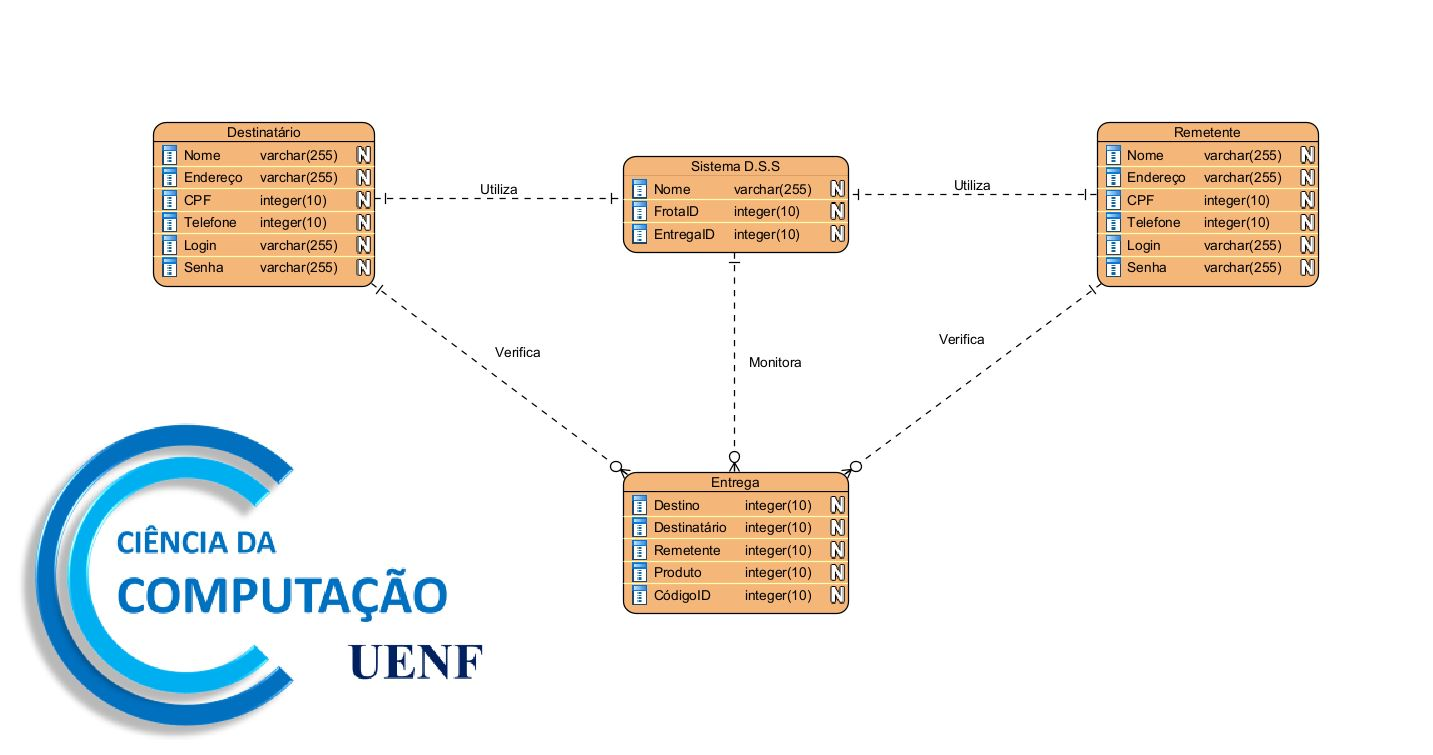
\includegraphics[width=1.2\linewidth]{Pictures/ER3}
	\caption{}
	\label{fig:er3}
\end{figure}

\section{Arquitetura do Sistema - Estilos}

    
    A arquitetura de um sistema desempenha um papel fundamental na determinação de como os vários componentes de um sistema interagem e funcionam em conjunto. A arquitetura de um sistema afeta diretamente nos diferentes aspectos do desenvolvimento, implementação e manutenção de sistemas. 

    \subsection{Arquitetura do Sistema}

	% TODO: \usepackage{graphicx} required
	\begin{figure}[H]
		\centering
		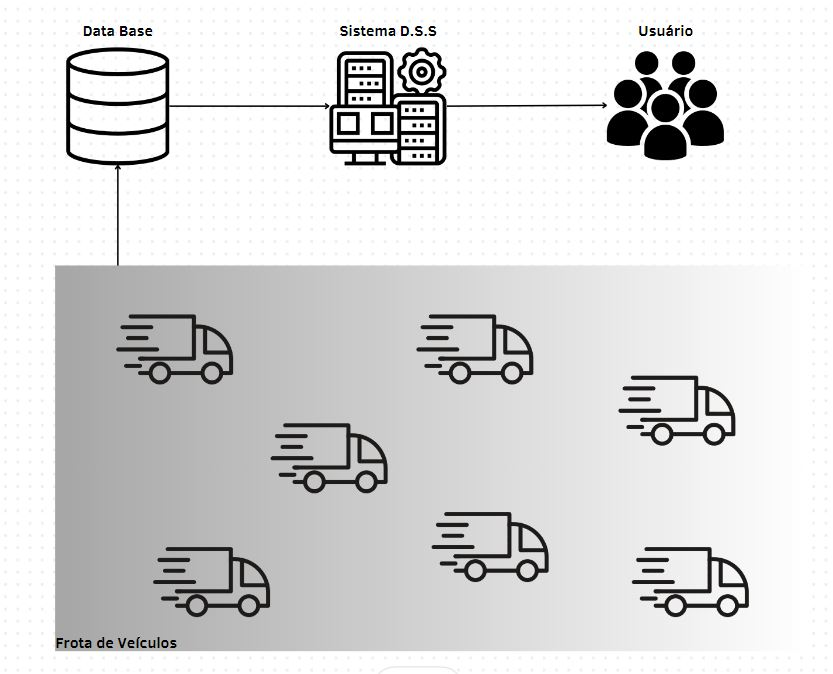
\includegraphics[width=1.2\linewidth]{Pictures/Arq0}
		\caption{}
		\label{fig:arq0}
	\end{figure}

    \subsection{Arquitetura do Hardware}

	% TODO: \usepackage{graphicx} required
	\begin{figure}[H]
		\centering
		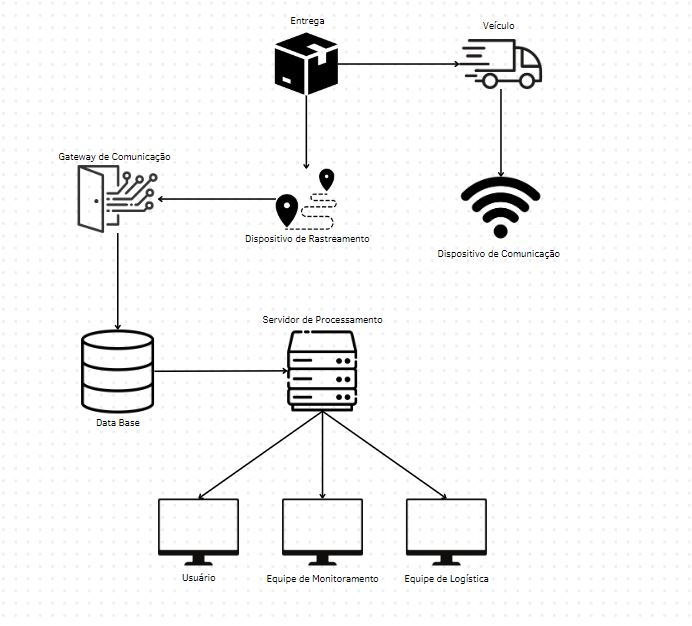
\includegraphics[width=1.2\linewidth]{Pictures/Arq2}
		\caption{}
		\label{fig:arq1}
	\end{figure}

    \subsection{Arquitetura de Software}
    
	% TODO: \usepackage{graphicx} required
	\begin{figure}[H]
		\centering
		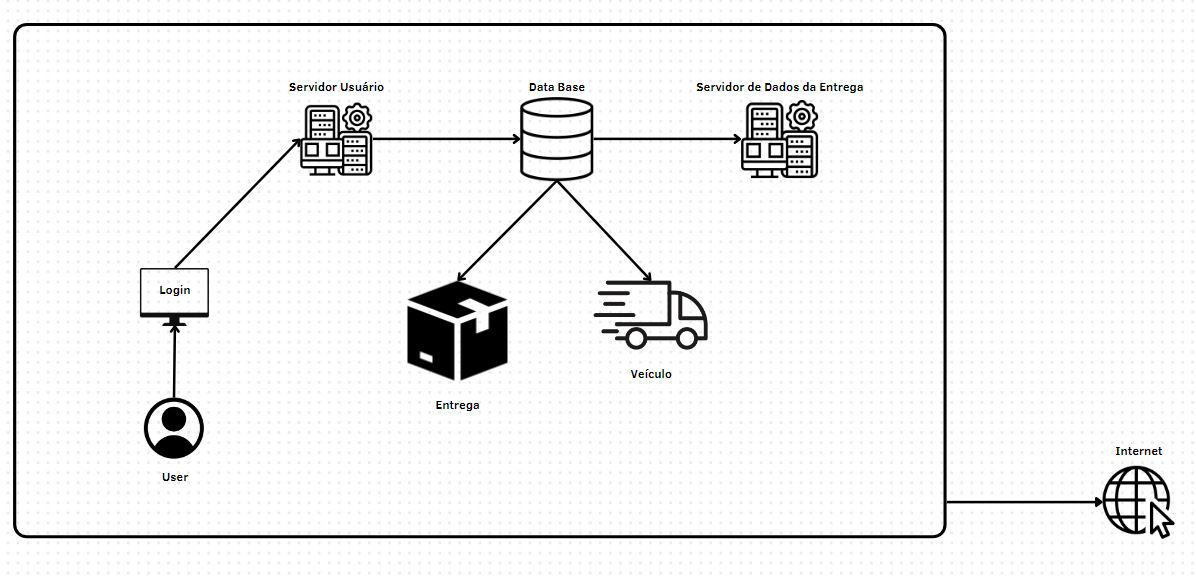
\includegraphics[width=1.2\linewidth]{Pictures/Arq1}
		\caption{}
		\label{fig:arq2}
	\end{figure}


